\documentclass[]{ctexbook}

\usepackage[a4paper,left=2cm,right=2cm,top=2cm,bottom=2cm]{geometry}
\usepackage[dvipsnames]{xcolor}
\usepackage[most]{tcolorbox}

\newcommand{\citebox}[1]{
    \begin{center}
    \begin{tcolorbox}[colback=gray!10,%gray background
                      colframe=black,% black frame colour
                      width=15cm,% Use 8cm total width,
                      arc=1mm, auto outer arc,
                      boxrule=0.5pt,
                     ]
    #1
    \end{tcolorbox}
    \end{center}
}


\title{COMPSCI 701 Note}
\author{Bo Pang/庞礴}
\date{Last Update: \today}

\ctexset{
    part/name = {Part},
    part/number = { \Roman{part}},
    chapter/name = {Chapter},
    chapter/number = { \arabic{chapter}}
}


\begin{document}
\maketitle
\tableofcontents

\part{Week 1-6}
\chapter{Creating Maintainable Software}

产品的\textbf{生命周期成本}是指产品生命周期内(从最初构思conceived到退役retired)的所有费用
(以金钱、精力、时间或其他方式衡量)的总和。\textbf{软件维护}是指保持软件产品有用性的活动。
研究表明,产品生命周期内的大部分费用发生在产品首次交付之后。所以,减少维护活动的成本
将大大降低软件产品的生命周期成本。软件产品的\textbf{可维护性}是指对其进行维护活动的难易程度。
可维护性是软件\textbf{质量}的一个方面。

\section{Maintainablity}
\paragraph{可维护性(Maintainability)}是产品的特性或属性,它影响维护活动开展的难易程度。
代码的设计和编写方式对该属性有很大影响。它是对产品进行维护活动的有效性(effectiveness)和效率(efficiency)。

而维护是产品交付后进行的活动。通常描述为:
\begin{itemize}
    \item 纠正性 corrective - 消除缺陷
    \item 适应性 adaptive - 改变产品以适应变化的环境
    \item 预防性 preventative - 改进质量的某些方面
    \item 完善性 perfective - 改进其实用性的某些方面,包括增加新功能
\end{itemize}

许多活动都在交付前进行。

\paragraph{Quality} For developers, quality means be more efficient at creating software. Ex: cheaper, produce, develop, fix faster\dots

\citebox{A quality attribute is a [quantifiable] or testable property of a system that is used to indicate how well the system satisfies the needs of its stakeholders}

是软件质量的一个方面。 In this course, we define maintainablity including these \textbf{independent} sub-attributes: \textbf{Comprehensibility, Alterability, Testability}.

\citebox{
    The degree of effectiveness and efficiency with which maintenance activities can be carried out on the product. It includes these independent sub-attributes:
    \begin{itemize}
        \item Comprehensibility (Analysability) -- Degree of effectiveness and efficiency with which the implementation can be understood in order to conduct maintenance activities with confidence
        \item Alterability (Modifiability) -- degree to which a product or system can be effectively and efficiently changed without introducing defects or degrading existing product quality.
        \item Testability -- degree of effectiveness and efficiency with which test criteria can be established for a system, product or component and tests can be performed to determine whether those criteria have been met.
    \end{itemize}
    The capability to smoothly and successfully perform maintenance tasks on the given item is defined by its maintainability. This encompasses several distinct characteristics:
    \begin{itemize}
        \item Understandability (Analysability) -- The ease and quickness with which the internal workings of the system can be grasped to confidently undertake maintenance tasks.
        \item Adaptability (Modifiability) -- The extent to which changes can be made to a system or product both swiftly and effectively without causing issues or diminishing its current quality.
        \item Examinability -- The ease and precision with which testing benchmarks can be defined and executed for any system, product, or part, confirming the fulfillment of set standards.
    \end{itemize}
}

Note that: 1. They are independent: when we talk about alterability, we must assume comprehensibility is OK. 2. Maintenance happens even before delivery.

\section{Comprehensibility}



\subsection{Program Comprehension Model}

有些因素与与我们为使代码易于理解而做出的决定无关,例如:使用未知的语言,阅读代码的人的水平\dots 我们需要一种“剔除”这些因素的方法,以便在评估与可理解性相关的决策时,不受试图理解代码的人的影响。为此,我们需要能够描述理解的"含义",这就是\textbf{程序理解模型(Program Comprehension Model)}。

作用:PCM explains how comprehension happens, the main components, processes, and interactions between them. It provides a systematic way for making a decision between choices relating to writing comprehensive code.

\begin{figure}[h]
    \centering
    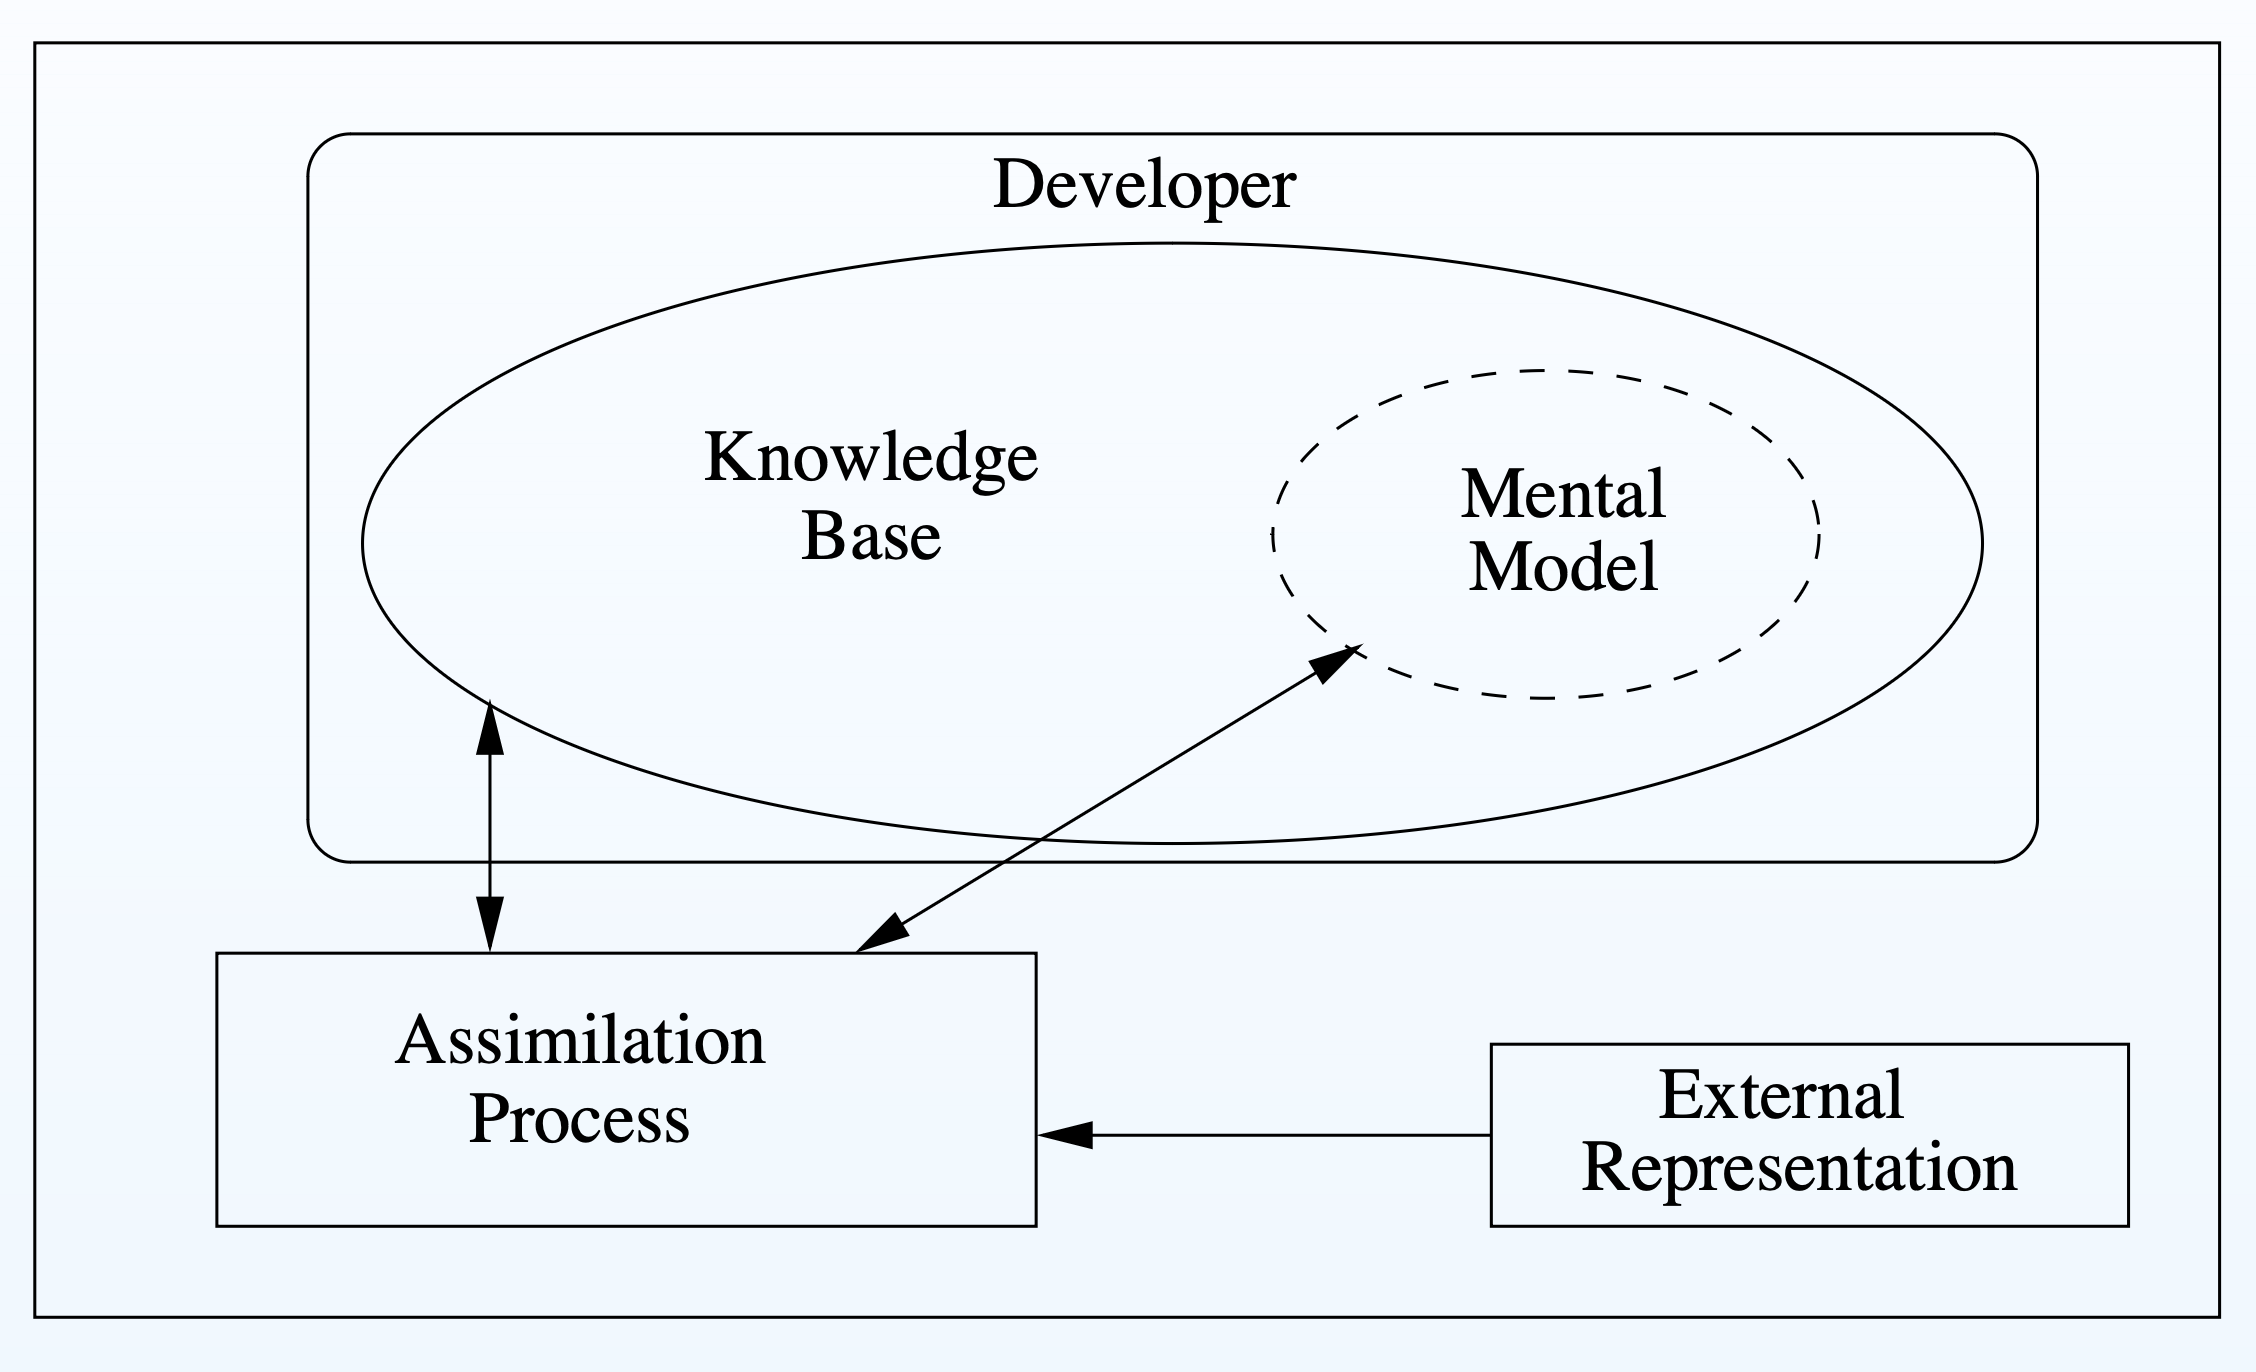
\includegraphics[width=8cm]{res/PCM.png}
    \caption{PCM by Michael}
\end{figure}

\begin{itemize}
    \item External Representation: e.g. source code, docs, peers\dots
    \item Knowledge Base: relevant knowledge that developers have already known, e.g. programming lang, domain knowledge
    \item Mental Model: current understanding, e.g. know parts, hypotheses
    \item Assimilation Process(内化过程): how to use all information to update the mental model, e.g. generation and verification of hypotheses
\end{itemize}

\subsection{可理解性与维护的关系}
可理解性关乎于开发者如何有效和高效地理解代码,以便有信心地进行维护活动。代码的可理解性与其维护性是紧密关联的。代码越容易理解,维护成本就越低,从而提高了代码的长期可维护性。
要提高代码的维护性,我们需要确保代码更容易、更快速且花费更少的精力去理解。

\subsection{如何评估可理解性?}

\paragraph{理解的有效性(Effectiveness)与效率(Efficiency)}要解释对一个实现的理解的有效性和效率,可以通过理解模型来实现,特别是考虑到同化过程的效果。

\paragraph{同化过程的有效性与效率}它取决于从知识库 (KB)、心智模型 (MM) 和外部表示 (ER) 中获取信息的效率和有效性。

\paragraph{信息的来源和理解难度的关系}信息的位置或来源对于理解来说非常关键。信息在心智模型、知识库还是外部表示中,这决定了理解的难度。

\section{Alterability}
\paragraph{可变性}是在不引入缺陷或降低现有产品质量的情况下,对产品或系统进行有效地和高效地改变的程度。

\subsection{Change Cases}
\paragraph{更改案例}描述了系统的潜在新需求或对现有需求的修改。它们的目的是预测和捕捉可能的更改,并指导系统的实现方式,以降低如果需要进行这些更改时的成本。

它们包括案例发生的可能性(Liklihood)和潜在的影响程度(Impact),可以视为系统演进的“用例”。

\subsection{评估可变性}
首先,需要确定实现应当适应哪些更改案例。
其次,针对这些更改案例评估实现。这意味着要查看系统或产品如何响应或适应这些特定的更改案例。

但请注意,有效和高效 "不包括与理解相关的成本
有些代码可能 "难以 "理解,但 "易于 "更改
因此,在评估可更改性时,应假设心智模型是 "完整的"(只要这样做是合理的)。

当一个更改案例的可能性较低时,它对可变性评估的影响也将较小。换句话说,如果预期某种更改的可能性非常小,那么在可变性评估中,我们不太需要考虑这种更改。当一个更改案例的影响较低时,它对可变性评估的影响也将较小。这意味着即使某种更改发生了,但如果其对系统或产品的实际影响较小,那么在考虑可变性时,我们不需要过于担心这种更改。我们应该主要关注那些\textbf{具有高可能性(Liklihood)和高影响(Impact)的更改案例},因为这些更改案例对可变性的影响最大。这意味着在设计和评估系统时,我们需要确保系统可以容易地适应这些具有高可能性和高影响的更改。

\subsubsection{评估影响}
对需求评估影响,而非现有代码。当评估更改的影响时,重点应该放在如何满足新的或修改后的需求上,而不是现有代码需要做多大的修改。影响是由现有系统的行为由于更改案例而改变的程度来决定的。例如,仅仅改变符号不会显著影响现有的行为,但改变游戏玩法会带来很大的差异。由于多种因素,评估更改的影响可能具有主观性,因此,可能难以为其提供一个精确的量化值。一种可能的方法是考虑你为这个更改案例准备支付的“原始成本”的比例。这种“成本”可以用财务、时间、努力或其他方式来衡量。通过这种方法,可以根据改变的大小和复杂性为其设置合理的预期。

\subsection{改变的位置和工作量}
在一个给定的更改用例中,对单个类中的代码进行所有必要的更改可能比在多个类中进行更改要容易。
原因:除了更改代码所需的时间,还有在不同类之间切换的时间。在类之间切换增加了出错的可能性。
在一个类中的单个方法中进行所有必要的更改可能比在同一个类的多个不同方法中进行更改要简单。
原因:再次涉及到在方法之间的切换时间。
在方法中更改一个语句可能比更改多个语句要简单。
原因:再次是因为切换。

进行“简单”的更改可能比进行“复杂”的更改要少工作。
例如,在switch语句中添加一个新的分支(该分支只对其他分支进行了简单的变种),与更改循环条件中的表达式相比。

\subsection{总结}
总之,可变性不是绝对的。软件或系统的可变性不是一个恒定或固定的属性。根据所需的更改类型,软件或系统的可变性可能会有所不同。

变更案例为评估可变性提供了一个方法,用于明确定义和描述可能需要对系统或软件进行的更改。它不仅描述了更改的具体内容,还可能包括更改的可能性和潜在影响。变更案例为评估和计划软件或系统的可变性提供了一个结构化的方法。这有助于确保可变性不仅基于直觉或主观判断,而是基于明确、详细和可衡量的标准。

一般来说,我们需要更改现有代码的次数越少,设计的可修改性就越高。
我们需要处理的地方越少(Efficiency)。
出错的可能性越小(Effectiveness)。

\section{Testability}
\paragraph{可测试性}测试性描述了为系统、产品或组件建立测试标准的有效性和效率,以及为确定是否满足这些标准而执行测试的能力。如果一个系统的测试性高,那么开发团队可以更轻松地定义测试标准,并验证系统是否满足这些标准。这可以确保软件的质量并减少缺陷。
\paragraph{测试}的主要目的是识别软件系统中的错误、缺口或未实现的需求。通过测试,开发者可以确保软件系统满足特定的测试标准或需求,从而确保产品的质量和稳定性。

根据测试标准(如性能、可用性、功能性)的不同,存在不同类型的测试。
系统测试:测试整个系统,确保所有部分和功能都按预期工作。
集成测试:确认独立开发的子系统能够协同工作。它关注的是接口和交互点,确保子系统之间没有冲突。
单元测试:针对单一的子系统或组件(如单个类)进行的测试。它通常关注特定功能的正确性。

手动测试涉及实人执行特定的测试用例,而自动测试使用脚本或其他工具自动执行测试。虽然手动测试在某些情况下可能更为直观和灵活,但自动测试通常更高效,尤其是对于需要频繁重复的测试。

测试涉及执行想要测试的代码,即被测实现(Implementation Under Test, IUT),并检查IUT的行为是否如预期。由于软件可能在各种条件下运行,因此需要在不同的条件下进行测试。这通常意味着为IUT提供不同的输入。

\paragraph{测试用例}是一组操作,通常由一组输入指定,对IUT执行以确定其是否导致正确的行为。

测试用例规定内容:
IUT:指定要测试的代码或模块。
预测试状态:这是执行测试之前IUT应处于的状态。
输入:要应用于IUT的数据。
预期状态或行为:这是在给定输入的情况下IUT预期的行为或输出。
执行测试用例的步骤:
预测试状态设定:确保IUT处于正确的预测试状态。
提供输入:根据测试用例的指定,为IUT提供输入数据。
执行IUT:使用给定的输入运行IUT。
结果验证:将IUT的实际行为与预期行为进行比较。这一步是判断测试是否通过的关键。

良好测试用例的一些关键属性超越了基本的“提高检测缺陷的概率”。为了确保软件的质量和可靠性,设计和执行高质量的测试用例是至关重要的。快速(Fast):
效率:快速的测试用例可以在短时间内执行,这意味着可以更频繁地运行它们,从而更早地检测到潜在的问题。
意义:如果测试用例执行速度快,那么在持续集成和持续部署的环境中,它们更有可能被频繁运行,这有助于提早捕捉和修复缺陷。
独立(Independent):
有效性:如果测试用例之间存在依赖关系,那么测试用例的执行顺序可能会影响结果,从而增加了出错的概率。
效率:
理解依赖关系需要额外的时间和努力。
如果某些测试用例依赖于其他测试用例,那么在执行特定测试之前,可能需要先执行其他测试,从而增加了测试的总体时间。
简单(Simple):
有效性:简单的测试用例降低了设计和执行出错的可能性。
效率:简单的测试用例往往执行速度更快,并且更容易理解,这也可能增加了测试用例的独立性。
可重复(Repeatable):
有效性和效率:
可重复性确保每次运行测试用例时都使用相同的预测试状态和固定输入,从而保证了一致性和可靠性。
这意味着测试用例的结果在不同的执行之间是一致的,从而提高了测试的准确性。

手动测试比自动化测试花费更长的时间,导致效率较低。由于手动测试时间较长,常常有将多个测试组合在一起的倾向,从而降低了测试的独立性和简单性。这可能会导致难以确定特定的缺陷来源和复杂的测试逻辑。手动测试的可重复性较低,因为执行每次测试时可能会有些许的变化,如人为错误、不同的执行顺序等。自动化测试在初始阶段可能会有较高的设置成本,但一旦建立起来,其后续成本就会降低。相反,手动测试的成本随着时间而持续累积,因为每次都需要人工介入。

自动化测试工具:
单元测试:
这是最基本的测试层级,针对代码的小部分(如一个函数或方法)。
工具:目前有很多“X-Unit”测试框架可用,例如JUnit(Java环境中的单元测试工具)。
集成测试:
测试多个子系统或组件是否能正确地一起工作。
工具:有一些工具可以用来进行集成测试,例如Mock测试工具,它可以模拟部分系统来进行集成测试。
系统测试:
测试整个系统的功能和性能。
工具:通常为特定系统定制,因为它涉及到完整系统的全面测试。

\paragraph{测试标准}是一组规则,这些规则定义了测试用例集(或称为测试套件)必须满足的要求,以便实现正在测试的(Implementation Under Test, IUT)被视为可接受的。测试标准提供了一个明确的、可衡量的方法,以确定系统、组件或功能是否满足预定的质量标准或要求。它们是质量控制过程中的关键组件,帮助确保软件产品的质量、性能和可靠性。

\paragraph{分支覆盖率}是一个常用的软件测试标准,要求在测试套件中的至少一个测试用例执行IUT中的每一个分支。这确保了代码中的每一个决策路径都被测试过,从而提高了发现潜在缺陷的可能性。

\paragraph{测试用例}是对如何测试特定功能或条件的明确规范,它通常包括前置条件、输入、期望的输出以及后置条件。

一个私有方法,这意味着它不能被类外部的代码直接访问。这对测试来说是一个问题,因为直接测试私有方法通常较为困难。测试人员需要找到一个方法来间接地测试它,例如通过一个公共方法。这会增加测试的复杂性。分支覆盖率要求每一个代码分支都至少被执行一次。这就需要为它的调用者方法选择适当的输入值,以确保方法中的每一个分支都被触发和测试。
这是一个复杂的任务,因为你需要深入了解代码的工作方式,以及哪些输入会触发哪些分支。

将方法从私有更改为公共可能会暴露类的内部细节,从而增加代码的脆弱性或违反面向对象设计的原则。

如果测试结果需要手动检查,那么这个过程会非常繁琐,并且效率低下。
手动验证测试结果也更容易出错,因为人们可能会遗漏某些细节或误解预期的行为。

\subsection{提高测试性}
测试的主要目的是为了模拟各种输入,观察并验证输出结果是否满足预期。为了实现这一目标,我们需要确保软件或系统的控制性和可观察性。

\paragraph{控制性 (Controllability)}涉及到我们能够如何控制或操作一个系统、组件或功能的能力。换句话说,我们需要能够按照我们想要的方式提供输入或触发条件。提高控制性意味着要确保测试人员或测试工具能够轻松地为软件或系统提供预期的输入或条件。

\paragraph{可观察性 (Observability)}
涉及到我们能够观察或看到一个系统、组件或功能的实际行为或输出的能力。为了有效地进行测试,我们需要能够清晰地看到软件或系统的行为,以便与预期的结果进行比较。
提高可观察性意味着确保输出、日志、状态或任何其他与软件或系统的行为相关的信息都是可访问和可理解的。

\subsubsection{设计上的实现}
如果系统具有结构化和功能明确的类,则测试者可能会更容易地控制和观察系统的各个部分。类的粒度和职责划分对于控制性和可观察性都至关重要。如果一个类提供了功能明确、有用的公共方法,那么它的行为和状态将更容易被控制和观察。公共方法为外部提供了与类交互的接口。选择合适的类和方法可以显著提高系统的测试性。开发者需要仔细选择和设计类及其方法,以确保它们对测试活动有利。

虽然增强控制性和可观察性是有益的,但过度的控制性和可观察性可能会导致其他问题。例如,过度的可观察性和控制性可能会破坏封装,从而增加系统的复杂性和引入潜在的错误。

\subsection{总结}
要提高系统或软件的测试性,一个关键策略是提高其控制性和可观察性。当这两个方面都很好时,测试过程将更加顺畅,能够更容易地识别和定位问题。



\chapter{OOD}

很多关于“OO”的讨论主要集中在语言的特性上。
是否可以独立于任何编程语言来讨论面向对象设计?
这是一个深入的问题。从纯理论的角度看,面向对象的原则和概念(如封装、继承和多态)是独立于具体语言的。但在实际应用中,某些语言的特性可能会影响或指导面向对象设计的实践。
我们必须具备哪些为OO语言讨论的特性?
这个问题留给读者去思考。常见的OO语言特性包括封装、继承、多态和抽象。但是,不同的人可能会对这些特性有不同的看法,取决于他们的经验和使用的语言。


\section{面向对象编程的基本特性}
\begin{itemize}
    \item 对象:面向对象编程的核心是对象,它们表示现实世界中的事物或概念,并具有属性和方法。
    \item 封装:封装是将数据(属性)和对该数据的操作(方法)包装在一起的概念。封装隐藏了对象的内部表示,并仅通过对象的接口暴露其行为。这提到了“封装了什么?”的问题,答案是“对象”。
    \item 类:类是创建对象的模板或蓝图。但是,不是所有被认为是OOP的语言都有类的概念,例如Self和JavaScript,它们使用基于原型的继承。
    \item 继承:继承允许新的类继承现有类的属性和方法。但这提出了一个问题:“什么是继承?”。例如,Emerald语言中的继承可能与其他语言中的继承有所不同。
    \item 类型:类型定义了一组值和这些值上的操作。例如,Smalltalk是一种动态类型语言,这意味着它在运行时检查类型,而不是在编译时。
    \item 泛型类型:泛型类型允许编程人员为一个类定义多种数据类型。这在Smalltalk中可能不太明显,而在Java的早期版本中,泛型是不存在的。
    \item 多态:多态允许不同的类的对象通过同样的接口进行交互。它也被称为虚函数调用、动态调度或消息发送。
\end{itemize}

仅仅使用一个具有面向对象特性的语言并不意味着你正在进行面向对象的编程。真正的OOP需要遵循某些设计原则和模式,而不仅仅是使用某种具有OOP特性的语言。

当执行面向对象程序时,它会创建相互发送消息的对象。面向对象设计描述了一个面向对象程序的设计或结构。

\subsection{面向对象设计的后果和影响}
封装:封装是对象间交互只能通过消息发送而产生的结果。这意味着,直接访问对象的字段或属性并不是面向对象的,因为真正的面向对象交互应该通过消息传递来完成。
继承:继承本身并不是决定一个程序是否为面向对象的关键,但它对设计质量有很大的影响。主要的原因是继承可以避免代码的重复,提高代码的重用性。
类型:类型的存在主要是为了防止某些类型的错误,例如变量的类型错误。
静态成员:静态成员不是面向对象设计的一部分,因为它们不属于特定的对象实例,而是属于类。
\textbf{类:类是用来描述和创建对象的。类是面向对象设计中的蓝图或模板,用于创建对象。}

因此,决定应该有哪些对象是创建一个可维护的面向对象设计的基础。换句话说,为了创建一个成功和可维护的OOD,开发者首先需要确定他们想要在系统中表示的实体或对象。

\section{类}
“类”是面向对象范式的核心概念。
类是面向对象设计的基础。
大多数自称为“面向对象”的编程语言都有某种形式的“类”结构。

设计过程中需要做的决策之一是决定包含哪些类。
类的选择确实会影响设计的可维护性。
为什么?类定义了系统的主要结构和行为。一个合理、结构化且有意义的类选择可以增加代码的可读性、可理解性和可扩展性,从而提高整体的可维护性。

\subsection{可维护的类}
\subsubsection{可理解性}
选择与我们已知知识相关的类会更容易理解。我们更容易理解与我们现实生活经验或已知领域知识相符的概念。所以,类应当与待解决问题的实际上下文有关,这样它们就会“有意义”。
\subsubsection{可变性}
为一个变更案例需要改动的越少,工作量就越小。在设计时考虑未来的可能变动并创建灵活性高的类可以降低未来维护的成本和风险。例如,如果一个类的功能高度集中且与其他部分的耦合度(coupling degree)低,那么它就更容易进行修改。
\subsubsection{可测试性}
如果可以更容易地查看和控制当前状态,那么测试的效率就会更高。设计类时应考虑到未来的测试需求,确保可以方便地访问和修改它们的状态。

\section{对象}
\subsection{对象的基本特性}
\begin{itemize}
    \item 身份 (Identity):每个对象都有一个独特的身份,区别于其他对象。
    \item 状态 (State):对象具有描述其当前条件或信息的属性。
    \item 行为 (Behaviour):对象可以执行的功能或方法。
\end{itemize}

\subsection{对象间的交互}
对于一个对象来说,想要向另一个对象发送消息,它必须有某种方法来识别那个对象。这里的“识别”即涉及到了对象的“身份”。
发送消息的真正价值在于接收方对象如何回应该消息,以及基于其历史或状态的响应方式。这里包含了两个重要概念:
响应或行为:当一个对象收到消息后,它会如何行动或响应,这涉及到“行为”这一特性。

历史或状态对象的当前状态或之前的历史状态可能会影响其对消息的响应。例如,一个关闭的窗户对象收到“打开”消息时的响应与一个已经打开的窗户对象收到同样的消息时的响应是不同的。这涉及到“状态”这一特性。

\subsection{可维护的对象}
不是所有对象都适合解决特定问题,因此,选择恰当的对象非常重要。Arthur J. Riel的启示是“尽可能模拟现实世界”。这意味着,设计应该基于真实世界的实体和关系。这可以使设计更有意义,更易于理解。Christensen的方法是首先确定行为(责任),然后将它们分组成角色,定义角色之间的协作模式,最后确定可以扮演这些角色的对象。这提供了一个从抽象到具体的结构化方法,从行为的责任到实现这些责任的具体对象。Booch提到对象是现实世界实体的抽象,代表了特别的“密度和内聚”的信息集群。换句话说,好的对象设计应当内聚,并且相关信息应当集中。Barnes和Kölling的建议是查看需求或描述,然后识别名词和动词。名词通常对应于类和对象,而动词对应于对象的行为或方法。这提供了一个直观的方法来从需求中提取设计元素。\textbf{设计的对象应该真实地反映它们所代表的现实世界实体的行为。这样可以确保设计与实际需求保持一致。}

当对象与真实世界中的某些东西对应时,如果我们已经知道这部分真实世界(它存在于我们的知识库中),那么这些对象将更容易理解。这减少了为理解代码意图而花费的时间和努力。如果对象代表真实世界中的实体,并且这个实体没有发生变化,那么这些对象也不应该改变。这种一致性确保代码的稳定性和可靠性。如果对象与真实世界中的某物相对应,那么我们应该能够像在真实世界中那样测试它们。这使得验证代码行为变得更为直观和实用。

\subsubsection{创建好的对象}
并非描述中的所有名词都对应于我们需要构建的东西。例如,描述中的“维基百科关于Kalah的文章”并不意味着需要一个与Wikipedia或Kalah文章相对应的对象。

并非描述中的所有名词都对应于我们需要构建的东西。例如,描述中的“维基百科关于Kalah的文章”并不意味着需要一个与Wikipedia或Kalah文章相对应的对象。

在设计中,可能会出现一些不是任何需求描述部分的合理 sounding objects,例如HashMap。这些通常是为了实现某些功能或性能需求而引入的。

所有建议都指向选择与要解决的问题有关的对象。选择与问题域紧密相关的对象可以提高代码的可读性、可维护性和可扩展性。

\subsubsection{Context Schema}
Context schema 指的是设计者对问题上下文的所有认知和信仰。换句话说,这是设计者关于问题背景的心智模型或视觉。例如,提到了“Noughts and Crosses”是在一个3x3的网格上进行的。这提供了一个清晰的上下文,帮助我们理解游戏的基本规则和环境。

上下文模式为设计师提供了一个基本的框架或参考,帮助他们了解和描绘问题的背景。只有充分了解上下文,设计师才能有效地开展工作并制定相应的策略。
\subsubsection{Design Schema}
Design Schema 是关于可能的设计构件的多样性的所有认知,包括设计决策和候选解决方案。这是设计者关于设计对象及其可选方案的心智模型。例如,设计者知道下拉菜单是一种为用户提供选择的紧凑方式。这种认知来自于过去的经验或学习,告诉设计者如何在特定上下文中提供用户界面选择。

设计模式为设计者提供了一种方法,帮助他们认识到不同的设计元素、策略和解决方案。这种模式可以指导设计师如何在给定的上下文中选择最佳的设计策略。

一个好的面向对象设计应该包含与上下文模式相关的对象(show respect to the context schema)。当类更接近于上下文模式或设计模式中的概念时,它的可维护性会更好。设计中的类若能紧密匹配现实世界的概念和设计者的认知,那么在未来对这个类的维护和理解就会更加直观和简单。如何确定一个类“正确地”匹配了一个概念?匹配的一个方面是,创建的对象数量应该符合预期。这意味着,当我们设计一个类,并在程序中实例化它,那么这个类的实例数量应该是可预测和合理的。

\chapter{Naming}

从我们已知的信息源(KB, 知识库)中提取信息并存入短期记忆(MM)比从外部参考中获取新知识更为高效。这意味着对于那些我们已经知道的概念,我们更容易理解和记忆。访问短期记忆(MM)比访问知识库(KB)更高效。这意味着,对于我们刚刚遇到或刚刚学习的信息,我们能够更快速地回想和处理。最后一个假设指出,访问知识库(KB)比访问外部参考(ER)更为高效。对于已知信息的回忆和处理速度比新知识的获取要快。

如果一个名称能够让我们更好地记住它代表的是什么,那么这个名称很可能会被更好地记录在短期记忆中,并且通常需要更少地参考知识库或外部参考。
\section{使用有意义的名称}
\section{避免编码}
编码指的是按某种特定方式选择名称,以编码各种信息。这通常是为了使代码更易读或理解,但很多时候,它可能导致混淆或过度复杂。

\subsection{编码的例子}
变量命名的前缀:例如,一个将要保存整数的变量应该以i, j, k开头,但不应该以l开头。这种编码方式在某些编程风格中是常见的,但在现代编程实践中,这种风格已经过时,因为它可能导致混淆。
字段名称前缀:所有字段名称都应该以f开头。这是另一种编码示例,但同样,这种编码方式可能会使代码变得难以阅读。
颜色编码:所有字段应该被染成特定的蓝色阴影。但这提出了一个问题:应该选择哪种蓝色?这种方法在视觉上可能有帮助,但如果没有明确的颜色代码,可能会导致混淆。
匈牙利表示法(Hungarian Notation):这是一个特定的编码例子,它在Microsoft Windows的C API中被使用,因为在那时基本上没有类型检查。例如,"arru8NumberList" 这个变量名编码了该变量是一个8位无符号整数数组。

\subsection{编码的问题}
虽然编码的初衷是为了提高代码的可读性,但实际上它可能会引起混淆,尤其是在没有明确规则或者团队成员对规则不熟悉的情况下。
编码可能导致不必要的复杂性,使代码更难维护。

\section{总结}
选择易于添加到 MM 中的名称,或易于在知识库中找到的名称。


\chapter{Formatting}

\section{Readability}
阅读性是指读者能够理解书面文字的容易程度。在自然语言中,文本的阅读性取决于其内容(词汇和句法的复杂性)和其展现方式(例如字体大小、行高和行长度等排版方面)。单词的长度(字符数量)、单词的结构(音节)以及单词的熟悉度(之前是否见过这些单词)都会影响阅读性。

代码的可读性是理解性的一部分。在自然语言中,阅读和理解是不同的——对于源代码来说,我们可能需要区分这两者。

识别元素(例如循环体)或区分元素(例如一个变量与另一个变量)的难度越大,或确定哪些元素属于一起的难度越大,阅读的难度就越大。
如果代码难以阅读,那么理解它的有效性和/或效率就会降低。也就是说,较低的可读性导致较低的理解性。
但是,易于阅读并不意味着一定容易理解!

\section{Formatting}
格式化的规则通常影响可读性,从而也影响理解性。

\paragraph{可读性}是指代码中的元素可以被识别和区分的程度。

\subsection{Vertical Formatting}

垂直格式化关注的是代码文件的结构和内容的垂直布局。这包括文件的大小、内容在文件中的顺序、以及空行如何提供视觉提示。

\subsubsection{文件的大小}
根据Martin的观点,一个理想的代码文件大约应包含200行代码,但最多不超过500行。
这种推荐是基于可管理性和可读性的考虑。较小的文件更容易理解,也更容易维护。
\subsubsection{文件内的顺序}
新闻隐喻(“倒置金字塔”):这是指在新闻报道中,最重要的信息放在最前面,随后是较为次要的细节。在代码文件中,这意味着主要或核心的功能和概念应该在文件的顶部,而较为次要或细节性的内容应该放在下面。

密切相关的概念应该保持接近:这可以减少滚动,帮助开发者快速找到和某个概念相关的所有信息。

函数调用的顺序:在一些编程风格中,被调用的函数应该在调用它的函数的下面。这样做的目的是为了在读者阅读代码时,他们可以顺序地了解函数的调用流程。
\subsubsection{空白行}
空白行在代码中作为视觉提示,帮助区分不同的“概念”或代码块。例如,可以使用空白行来分隔函数、方法或不同的逻辑块。
这提高了代码的可读性,使代码更加结构化和整洁。

\subsection{Horizontal Formatting}

水平格式化关注的是代码在同一行内的布局和结构,如行宽、空白和缩进。

\subsubsection{行宽}
Martin推荐每行代码字符数为45。这考虑了阅读的舒适性,确保代码在一屏内可见,减少滚动和横向滚动。
\subsubsection{使用空白}
通过增加或减少空格,可以表示代码元素之间的关系有多紧密。例如,操作数和操作符之间的空格可以使表达式更易读。
\subsubsection{缩进}
缩进是代码层次结构的关键部分,用于表示块、循环和条件语句的起始和结束。它帮助读者理解代码的流程和逻辑结构。


\chapter{Comments}

\section{Good or Bad Comments}

代码异味(Code Smells)是指在代码中可以观察到的某些迹象,它们可能意味着背后存在更深层次的问题。这些不是错误——代码仍然可以运行——但它们暗示了设计上的不足,可能使代码难以维护和拓展。

Martin提到的“注释作为遮掩”的代码异味,强调了一个观点:如果代码需要大量注释来解释,那么它可能没有很好地表达自己的意图。优秀的代码应该是“自解释的”(self-explanatory),这意味着通过良好的命名和结构设计,代码应该尽量清晰和易于理解,而不是依赖注释。

但这并不是说所有的注释都是坏的。有时,注释是必要的,例如当解释某个复杂算法的原理或背景时,或者解释某些代码为什么要采取非常规的做法时。关键是区分何时应该使用注释,何时应该通过重构代码来提高其可读性和清晰度。

马丁以及很多其他人为什么对注释持负面态度?甚至好的注释也会带来额外的工作:
需要编写注释,这本身就是工作。
如果注释描述了代码的内容,并且代码发生了变化,那么注释至少需要被检查以确保它们仍然与代码保持一致(在最坏的情况下,需要修改注释)。
如果注释没有描述代码的内容,那么它们存在的意义是什么?
因此,注释最好能提供一些价值,通常是提高代码的可维护性。
它可以改善“同化过程”:不必阅读太多的代码,不必过多地思考代码可能的意义。

好的注释包括:法律、信息性、意图、澄清、后果、待办事项、扩展、API文档(例如Javadocs)。
不好的注释有:喃喃自语、冗余、误导、强制、日志、噪声、可怕的噪声、位置标记、属性、被注释掉的代码、HTML、非局部信息、过多的信息、不明显的联系、函数头。

有一件事你永远无法在代码中做到,那就是解释没有采取的路径。
当有多种方法可以做某事时,有人可能会看到该选项并想知道你为什么没有选择另一种选项——在注释中解释。

\section{Explain yourself in code}
选择一个描述性强且容易理解的变量名可以使代码更加高效。这是因为代码的阅读者不需要经常回到变量的声明部分,或者查看注释来理解变量的意义。
描述性的变量名可以减少对外部表示的依赖,增强代码的自描述性,从而使得代码理解的过程更加流畅和直观。
一个具有描述性的变量名可以帮助维护者快速建立和更新其心智模型,从而更高效地理解代码的功能和意图。

\section{注释的作用}
代码的开头有一个文档化的注释,解释了该方法的功能——给定一个数n,返回其对应的斐波那契数列中的数。此外,该注释还描述了方法的参数和返回值。
代码内部的注释提供了关于代码如何实现其功能的更多详细信息。

对于一些不那么直观的代码部分,注释可以帮助读者更快地理解代码的意图和功能,而无需深入分析代码的每一个部分。

考虑两种情况:一种是读者阅读注释来理解代码,另一种是读者通过仔细分析代码来重建代码的意图。
虽然两种情况都需要访问代码的外部表示(ER),但是没有注释的情况下,读者可能需要更多的时间或更深入地理解代码的各个部分,从而推断出代码的意图。因此,没有注释的情况下,理解代码的过程是不够高效的。

虽然注释很重要,但不必要的或冗余的注释会增加阅读和理解代码的工作量。例如,对于经验丰富的开发者来说,解释Fibonacci数列如何计算可能是多余的。
试图理解代码需要阅读这些注释以及它们解释的代码,如果注释是冗余的,那么这会使得理解过程更为复杂。

\section{Other comments practices}
\subsection{注释掉的代码}
有时,开发人员在修改代码时可能会注释掉某些部分,而不是完全删除它们,这通常是出于在将来可能再次需要这些代码的考虑。

分析:这种做法不推荐。一旦代码被注释掉,其他开发人员可能不敢删除它,因为他们不确定是否会再次需要这些代码。这最终会导致代码库中充斥着未使用的、注释掉的代码,增加了代码的复杂性和难以维护性。

\subsection{闭括号注释}
有时,开发人员在一个长方法或代码块的闭括号后面添加注释,以表示这个闭括号是结束哪个部分的。

分析:如果你觉得需要在闭括号后面添加注释,那么这通常意味着你的方法或代码块太长了。长代码块往往难以理解和维护。为了提高代码的可读性和维护性,应该考虑将代码块拆分成更小、更具有描述性的部分。
\subsection{位置标记}
位置标记通常用来在代码中标记特定的段落或部分,以方便其他开发人员快速导航。

分析:如果你觉得需要使用位置标记,那么这通常意味着你的类或方法太长了。如同闭括号注释的情况,过长的类或方法应该被拆分以提高代码的清晰度。
\subsection{TODO注释}
开发人员经常使用TODO注释来标记代码中尚未完成或需要进一步改进的部分。

分析:这些TODO注释有时被称为“自承认的技术债务”。它们表明代码在某些地方是不完整或不完美的。长期存在的TODO可能意味着项目中存在着悬而未决的问题或需要进一步的优化。
\subsection{注释作为沟通形式}
注释是开发人员之间关于代码意图、设计决策和功能的通信工具。

分析:由于注释是为人类(而不是机器)阅读的,因此它们应该是高质量的,能够清晰地传达必要的信息。质量差的注释可能会误导开发人员,导致他们对代码的错误理解。

\section{总结}
尽可能避免使用注释。支持理解的注释(可能还包括可维护性的其他方面)是可以接受的。

\chapter{Functions}

代码分解思想起源于1940年代或更早。这意味着,即使在计算机技术尚未普及,程序设计初期,这种方法已经开始受到认可。最初采用这种方法的目的是为了减少代码重复和内存使用。这可以理解为,早期计算机资源有限,因此节约内存和减少冗余是至关重要的。1960年代或更早,为了使代码更容易维护,开始有了将代码分解为单独可调用单元的想法,这一概念与“结构化编程”相对应。
结构化编程强调使用一种模块化、可预测的方式编写代码,使其易于阅读、维护和调试。这种思想与简单地节约资源或减少重复相比,更侧重于代码的清晰度和长期可维护性。它基本上是对“go to”语句的有纪律的使用。
结构化编程强加了关于代码组织方式决策的更多规律。如今的编程语言,如果有“go to”语句,只是以非常受限的形式存在,例如条件、循环语句。

结构化编程禁止在任何函数中有多于一个的返回。

\section{Functions should be}
小型(Small):函数应该尽量小而简洁,这样更容易理解和维护。

做一件事(Do One Thing):这也称为“内聚性”(cohesion)。一个函数只应该做一件事,并且做得好。

函数的每一层都应该有一个抽象层次(One Level of Abstraction per Function):函数内部的所有语句都应该在同一层次的抽象上。这可以确保函数易于阅读和理解。

从上到下阅读代码(Reading Code from Top to Bottom):函数的组织和呈现方式应该让读者能够从上到下顺畅地阅读。

使用描述性名称(Use Descriptive Names):为函数选择有意义的名称,这样可以清楚地描述其功能和用途。

函数参数(Function Arguments):函数的参数数量应该有限,每个参数都应有明确的目的。

没有副作用(Have No Side Effects):函数不应该有任何意外的副作用,例如修改全局变量或更改传入的参数的状态。

为了获得高质量的函数:

首先避免问题(Avoid problems in the first place):在编写代码时,一开始就遵循最佳实践,可以预防大多数问题。

如果出现问题,重构(If got problems, refactor):重构是一种技术,通过修改代码以提高其质量,但不改变其功能。

Pro 单一返回: 单一退出点可以使函数的控制流更可预测,从而简化心智模型。
反对单一返回: 对于较长的函数来说,在末尾设置单一返回点可能会迫使读者在心智模型中保留更多的中间状态,从而使代码更难理解。
知识库:
支持单返回: 具有结构化编程背景的程序员或受过避免使用多返回语句训练的程序员可能会发现单返回点更直观。
反对单点返回: 现代编程教育通常会强调提前返回和保护子句以提高清晰度,因此有这种背景的程序员可能更喜欢多返回。
外部表示法:
支持单一返回: 单一返回可能会导致更少的分支和更线性的 ER,这可能更容易理解。
反对单返回: 单一返回的函数可能需要更深的嵌套或增加标志变量,这会使ER变得杂乱无章,难以理解。
同化过程:
支持单返回: 如果由于单返回而使控制流更具可预测性,则可能加快同化过程。
反对单一返回: 如果实现单一返回会使代码更加复杂,则可能会减慢同化过程。

\subsection{Self Documenting}
使用小的函数来创建自文档的代码。也需要避免使用字面量。

\subsection{每个函数应该维持一个抽象级别}
Martin建议避免在同一个函数中混合“高级”概念和“低级”概念。
这种混合可能会导致代码难以理解和维护,因为函数不再遵循“做一件事”的原则。

高级概念可能涉及领域的核心概念,如“更改网格中的单元格”。这些是更接近业务逻辑或任务的核心目标的代码段。
低级概念可能涉及实现细节,如“数组中的值表示什么”。这些是处理具体数据结构或操作系统调用等具体细节的代码段。

如果一个函数同时处理高级和低级概念,那么它可能在功能上太过复杂。
这使得函数更难测试,更难理解,也更难修改。

识别函数中各个部分的抽象级别可能是一个挑战。
一种可能的方法是使用缩进级别作为启发式方法来识别。这个方法的基本思路是:更多的缩进可能意味着更低的抽象级别。然而,这只是一个简化的方法,可能并不总是准确。
尽管Martin提倡每个函数只有一个抽象级别,但他没有明确地定义什么是一个“抽象级别”。这可能会导致一些歧义和困惑,因为不同的程序员可能对“抽象级别”的理解各不相同。一个可能的启发式是2个缩进就已经足够。

代码的可读性如何得到提高?
重构后的版本中,playerMove函数更加简洁。主要的改进是将玩家移动的合法性验证部分提取到一个新的函数playLegalMove中。这种模块化使函数的逻辑更清晰,也更符合“每个函数只做一件事”的原则。
代码的减少与理解性:
减少了一些重复和冗余的代码,从而使吸收过程需要的时间更少。
通过使用具有描述性的函数名(如playLegalMove),当该名称有意义时,访问心智模型更为高效。
代码的进一步重构:
虽然playLegalMove函数确实提高了playerMove的可读性,但它本身仍然有与原始playerMove相同的嵌套级别。这意味着可以考虑对playLegalMove进行进一步的重构。

如果一个函数只包含一个抽象级别,那么它很可能是一个小函数。这意味着它不会包含太多不同的逻辑或功能。但这不是绝对的,因为一个函数可能有一种可以利用的规律性,使其在短时记忆中的需求减少,即使它的长度超过了典型的“小函数”。

\subsection{自上而下阅读}
在新闻报道中,"倒金字塔"模型是指最重要和最基本的信息出现在文章的开头,而细节和补充信息随后出现。这种写作方式确保了读者即使只阅读文章的一部分,也可以获得核心信息。相似地,代码也可以被组织成这种层次结构,其中顶部函数是最抽象的,而底部函数是最具体的。

按照这种组织方式,代码的第一个函数提供了一个高层次的概述,其中大部分内容是对其他更具体函数的调用。这种组织结构有助于初次阅读代码的人快速地理解代码的主要目标和结构

这种从顶部到底部的代码阅读策略有助于提高效率。程序员可能只需要阅读顶部的函数就能获得足够的理解,而不必深入到每个具体的函数。这样,他们可以更快速地理解代码的主要逻辑和功能。

当程序员遇到一个函数调用时,他们知道从哪里开始查找它的声明。如果代码按照从抽象到具体的方式组织,那么函数的声明很可能紧跟在其调用的后面,这也提高了查找效率。

\subsection{Do One Thing}
\paragraph{内聚性}是指一个模块或函数在功能上的一致性。当说到一个函数具有高内聚时,意味着它只做一件事情,并且做得很好。高内聚有助于使代码更加模块化、可维护和可读。

很难具体量化一个函数到底在做多少件事情。但一个好的起始点是,尝试描述该函数的功能,如果在描述中出现了“和”或“或”这样的词,那么这个函数可能正在做多于一件的事情。

一个只做一件事的函数很可能是小的,因为它的功能被限定并集中于单一的目标。
大的方法或函数可能会涉及多个功能,从而降低其内聚性。

做单一功能的函数带来了多种优点。
在首次阅读时更容易理解,因为它的目的和功能是清晰和有限的。
当再次遇到该函数时,更容易回忆起它的功能,因为其功能是明确和唯一的,无论其实际大小如何。

\subsection{使用描述性的名称}
如果一个函数确实只做一件事情,那么它的名称应该清晰地描述出它的功能。这样,当其他开发者或未来的你自己再次查看代码时,可以快速地理解该函数的目的和功能,而无需深入其内部实现。

尽管在许多场景下,简短性可能是理想的,但当涉及到代码的清晰性和可读性时,长名称可能更为有利。如例子中所示,gameOverWithWinner() 和 gameOverWithDraw() 这样的名称比简短的名称更有描述性,能更快地传达函数的功能。

做单一功能的函数往往更容易命名。这是因为其功能是明确和限定的,所以为其选择一个准确的描述性名称相对更简单。
当函数具有多重功能或其功能不清晰时,为其选择一个准确、简短且描述性的名称可能会变得更加困难。




\subsection{小的函数}

函数大小的重要性:Martin的主张是,函数应该非常小。他甚至建议函数不应超过4行。这可能听起来很极端,但背后的逻辑是,更小的函数更容易理解,因为程序员只需要在短时间内关注一小部分的代码。这也使得函数更容易测试和维护。
这个建议与人的短期记忆能力有关。研究已经证明,人的短期记忆只能容纳有限的信息。这意味着,当一个函数或代码段太长时,要理解它的所有部分,程序员可能需要多次查看和思考。而小函数则更容易一次性理解。



\subsection{关于参数}
Martin关于函数参数数量的观点:

零个参数(zero arguments):这是理想的情况,因为它意味着函数不需要外部信息来执行其任务。
一个参数(one argument):这是可以接受的,但是要避免使用标志参数(flag arguments),因为它们会使函数的功能变得不明确。
两个参数(two arguments):勉强可以接受。
三个参数(three arguments):应尽量避免。
超过三个参数:这意味着函数可能在尝试做太多的事情,应该考虑重新设计或拆分。
输出参数(output arguments):它们是待发生的问题,因为它们使函数有副作用,这可能会导致未预期的行为。

\subsubsection{为什么避免参数}

使用StringBuffer作为示例,Martin指出,如果我们把它作为参数传递,而不是作为字段(field),那么每次读到它时,读者都必须去解释它的含义。这增加了理解代码的难度。
当然,同样的问题也适用于字段。但字段通常更容易理解,因为它们在类或模块的范围内是已知的。
另外,从测试的角度看,参数更加困难。参数需要在每次调用时都进行设置,这可能会导致测试的复杂性增加。
然而,与参数相比,字段可能同样具有挑战性,或者更具挑战性。因为字段可以在类的多个地方被修改,这可能导致更多的不确定性和难以预测的行为。

\subsubsection{如何减少参数}
为减少函数参数数量而增加字段可能是一个糟糕的主意。字段存在是为了表示对象的状态。在面向对象编程中,对象的状态是由其字段来维护的。仅为了减少函数的参数数量而随意增加字段是不明智的。这可能导致对象状态的不必要复杂性,并可能违反了面向对象设计的原则,如封装。
如果增加字段并不真正代表对象的逻辑状态,那么这种做法可能会导致代码更难维护和理解。一个有关字段的启发式原则是:字段是否被公共函数(public function)所需要?这意味着如果一个字段只被私有方法使用,并且只是为了减少参数,那么它可能不是必要的。

参数对象是一种设计模式,它涉及到将多个参数封装成一个对象,从而减少函数的参数数量。这种方法在处理复杂函数和构造函数时尤为有用,特别是当它们需要多个参数时。
通过引入参数对象,可以简化函数签名,提高函数的可读性,并使得函数的调用更加直观。

有时,为参数创建一个明确的类并不是那么直观。例如,函数stillSearchingForFirstLetter接受三个整数参数,但并不清楚如何将它们组织成一个类或对象。
当函数的参数和逻辑不那么清晰时,这可能是一个设计或重构的迹象。即,这个函数可能需要进一步的思考,以确定其真正的目的和所需的参数。

\subsubsection{输出参数 Output Arguments}

函数修改了传入的参数,叫做输出参数。

Martin认为,输出参数可能会导致混淆,因为开发者通常不期望函数会改变传入参数的值。当函数修改其参数的值时,这可能会导致错误,特别是当开发者不清楚或不记得这一点时。

updateBoardWithMove函数中,参数houseChosenForMove的值被改变。虽然这种操作在技术上是容易实现的,但它可能会给读代码的人带来混淆。特别是当没有明确的文档或注释说明这一行为时。
然而,示例中的注释提到了houseChosenForMove的状态变化。这种注释的存在可能暗示了该函数存在设计上的问题。通常,如果一个函数的行为需要通过注释来解释,那么这可能是一个信号,表明这个函数的设计和行为可能需要进一步的优化。


\subsubsection{与PCM结合}
程序理解模型通常包括几个组件,如Mental Model (MM),Knowledge Base (KB),External Representation (ER) 和Assimilation Process。多个参数可能会影响这个模型中的Assimilation Process部分。
当一个函数有多个参数时,开发者需要在心智模型中跟踪这些参数和它们的交互,这可能会使代码更难理解。
多个参数意味着开发者在阅读和理解代码时需要在KB和ER之间进行更多的切换,这可能会降低效率。
总之,根据程序理解模型,多个参数可能会使代码的理解变得更加困难和低效。

\subsubsection{平衡参数数量}
我们可以看到参数对于函数的重要性以及过多参数带来的问题之间存在明显的矛盾。如何平衡这两个方面?

精确使用参数:确保每个参数在函数中都有明确的目的。避免添加不必要的参数。

参数组织:对于接受多个相关参数的函数,考虑使用对象或结构来组织这些参数,从而将它们组合为一个参数。

使用默认参数和函数重载:在某些编程语言中,可以使用默认参数或函数重载来为不同的使用情况提供不同的参数集,从而在不牺牲功能的情况下减少参数数量。

参数注释和命名:确保参数有描述性的名称并适当地注释,以提高其可读性和理解性。

\section{不要重复自己 DRY}
DRY原则是一种编程哲学,旨在减少重复的代码。重复的代码不仅导致代码膨胀,还可能导致维护上的问题。当一段代码被复制到多个地方,任何对该代码的修改都必须在所有地方进行,否则可能会导致不一致和错误。

代码重复通常会降低代码的可维护性。例如,如果开发者需要修改重复的代码,他们必须找到并修改代码的每一个实例,这会消耗更多的时间和精力。
当开发者需要阅读或理解代码时,重复的代码片段可能会造成困托。不必要地阅读相同的代码片段会浪费时间,并可能导致误解,尤其是当上下文略有不同时。

如果其中一个重复的代码片段发生变化,而其他地方的相同代码没有相应地改变,那么这可能会导致未预期的行为和错误。因此,即使初始的代码复制可能是出于快速实现的目的,但长期看来,这种做法可能会带来更多的问题。

删除重复的代码很可能会减少相关方法的大小。小型、简洁的方法更容易阅读和维护,这也符合之前讨论的关于方法应该小且只做一件事的原则。

\section{小函数真的利于维护吗}
小函数可以使代码更容易读懂和维护,因为它们通常关注于单一的功能或任务。但同时,太多的小函数可能导致难以追踪和管理。

编写小函数确实有成本,特别是当将大型方法分解为多个小型方法时。必须权衡这一过程的利与弊。例如,一个小函数可以提高代码的可读性,但同时也可能增加代码的复杂性,因为需要跳转到多个地方才能完全理解一个功能是如何实现的。

添加更多的小函数有时可以减少代码量,尤其是当它们能够消除重复代码时。然而,每个函数都有其开销(例如定义、注释、调用等),所以在某些情况下,增加更多的函数实际上可能会增加代码量。

Martin的建议基于经验,可以看作是一套启发式规则。而不是盲目地应用这些启发式方法,更重要的是理解它们为什么以及在哪些情况下有效。也就是说,应当理解每个建议背后的原因,以便在合适的情境下使用它。

\subsection{与PCM结合}
1. 提高代码的清晰度和可读性(Assimilation Process):

小函数一般都是围绕着一个特定的任务或功能。这使得开发者在通过ER理解代码时,可以更快速地将其与KB中的相关知识模式匹配,从而更快地形成MM。

2. 强化心智模型的清晰度(MM):

当每个函数都专注于一个单一任务时,MM变得更加清晰。开发者不需要花费大量的时间和精力去理解复杂的、执行多个任务的函数,这也可以帮助他们更好地预测程序的行为。

3. 减少认知负担:

在ER中,小函数的名称,如果命名得当,可以直接告诉开发者函数的目的和功能。这种自文档化的代码减少了从ER到MM的转化所需的努力。

4. 长期维护的价值:

当代码需要修改或扩展时,小函数提供了明确的界定,使开发者更容易确定哪部分代码需要修改。此外,它还可以减少出错的机会,因为修改的范围通常更小、更集中。
由于小函数的目的明确,它们也更容易被测试,从而增加了代码质量。

结论:
小函数确实可以使程序更容易理解,它们提供了明确的上下文,有助于开发者构建和维护心智模型。从长期的角度看,小函数确实为程序的维护带来了价值,特别是在团队环境中,它们有助于新成员快速地理解和参与到项目中。

\section{总结}
许多小的高质量函数可以帮助理解:
小函数的主要优势在于它们可以更明确地表达代码的意图。一个有描述性的函数名可以快速地告诉开发者该函数的功能,从而使代码自我说明。
例如,一个名为calculateTotalAmount()的函数可能比一个简单名为calculate()的函数更具描述性。后者可能需要查看函数的内部实现或调用上下文才能理解它的真正功能。

抽象级别的考虑:
当在阅读代码时,开发者可能不需要关心那些低抽象级别的功能(也就是更具体或低级别的操作)。这意味着,他们可以专注于高级逻辑,而不是被困在细节中。
这进一步减少了频繁参考外部表示(例如函数的具体实现或其他文档)的需要。从而可以更快速、高效地理解代码的主要逻辑和结构。

重构以改进函数的使用:
重构不仅仅是为了修复错误,它也是一个使代码更加整洁、更具可读性和可维护性的过程。
为了提高函数的效用,有时可能需要对现有的函数进行拆分、合并或重命名等重构操作。

分步进行重构:
在实际编程中,很少有一步到位的重构。相反,开发者通常会分多个小步骤进行重构,确保每一步都不会破坏现有的功能。
这种分步的方法还允许开发者在每一步都进行测试,确保代码的功能性不受影响。

使用许多优秀的小函数可以帮助理解(至少)。
因为它们的名称表明了它们所做的一件事(自文档化代码!)。
通常不需要考虑抽象程度较低的函数。
通常不需要考虑抽象程度较低的函数、
我们没有可靠的方法来确定大多数建议的成本效益比。


\chapter{Classes}

类应 "表示 "上下文模式或设计模式中的 "概念"。在编程中,概念通常指的是可以被建模和表示的实体或行为。如果一个类能够清晰、准确地捕获某个概念的核心属性和行为,并且没有多余的、不相关的信息,那么我们可以说这个类“代表”了这个概念。

\section{Martin on Classes}
\subsection{Organization}
一种基本的组织顺序如下:
\begin{itemize}
    \item ublic static final fields (constants):
          常量经常用于定义与类关联的固定值或配置。将它们置于顶部可以方便地看到这些重要的固定值,无需在代码中搜索。
    \item other static fields:
          这些字段通常与类级别的状态或配置有关,而与实例无关。与常量一起放在顶部,读者可以清楚地看到与整个类相关的信息。

    \item instance fields:
          实例字段是与特定对象实例相关的状态。放在静态字段后面,它们为后面的方法提供了上下文,因为这些方法可能会操作这些字段。

    \item Constructors:
          构造函数是用于初始化对象的方法。在实例字段之后放置它们是有意义的,因为构造函数通常会设置这些字段的值。

    \item public methods:
          公共方法定义了类的公共接口,即其他类或对象如何与其交互。它们应该根据其重要性或调用频率进行排序。

    \item non-public methods (but those called by public methods close to the methods they're called from):
          非公共方法通常是辅助方法或实现细节。它们应该被放置在被调用的公共方法附近,这样读者在阅读公共方法时可以轻松地找到它们。对于protected与private之间的排序,考虑到protected可能被子类使用,可以考虑将其置于private方法之前。
\end{itemize}

使用这种顺序的原因(仅供参考):

逻辑流程:此顺序遵循从一般到特定的逻辑流程。首先是与整个类相关的静态内容,然后是与实例相关的内容。

阅读流:开发者通常首先关注公共接口,即公共方法。将它们放在前面可以确保他们不必滚动到文件的末尾来查找这些方法。

聚焦核心功能:公共方法通常定义了类的核心功能,而私有方法提供了实现这些功能所需的辅助功能。将公共方法置于前面有助于突出显示核心功能。

易于维护:当你需要修改或添加一个功能时,相关的代码通常在彼此附近,这减少了在文件中搜索相关代码的时间。

\subsection{Encapsulation}

对象(及其所属的类)代表上下文或设计方案中出现的概念或抽象。在面向对象编程中,对象是现实世界概念的模型或表示。
字段描述对象的状态。这是对象的内部属性,它决定了对象在特定时间点的行为和特性。

封装的主要目的是隔离类的内部实现细节,使得外部代码不能直接访问或修改它。这样做的一个重要原因是,当内部实现发生变化时,不会影响到使用这个类的其他代码。私有字段和实用程序方法是这种隔离的关键组成部分。直接访问对象的实现细节或其内部状态是不良的设计选择。这是因为:
如果实现者更改了内部表示,那么所有直接使用它的事物都必须也进行更改,这会导致维护上的噩梦。
直接暴露实现细节会导致代码之间的强耦合,降低灵活性。

封装确实提高了代码的可理解性,因为开发者可以更加集中地理解对象的核心功能,而不是被其内部工作机制所干扰。
同时,封装也是可维护性的关键。当实现细节被封装,更改它们不会对使用该类的其他部分产生不良影响。

当我们希望子类能够访问或覆盖某个字段或方法时,受保护的可见性是可以接受的。尽管这为子类提供了更多的灵活性,但它也增加了父类和子类之间的耦合,这可能会降低代码的维护性。

公共字段可以被任何外部代码直接访问和修改,这违反了封装的原则。此外,公共字段不允许对其访问或修改进行任何形式的控制,例如数据验证。

有时,我们确实需要访问对象的某些内部值或状态,但关键是如何做到这一点。优秀的设计通常通过提供公共的getter和setter方法来实现这一点,这些方法可以控制对内部状态的访问和修改,而不是直接暴露字段。

用字段和方法的可见性来解释 "良好封装 "是不够的:封装不仅仅是关于字段和方法的可见性。它也关系到如何组织代码、如何定义类和对象之间的交互以及如何管理依赖关系。只关注可见性可能会忽略这些更深入的考虑。

将字段和实用方法私有化:

安全性:私有字段和方法只能被类自己使用,这意味着开发者不必担心外部代码错误地使用或修改它们。

清晰的接口:当字段和实用方法被设为私有时,类的公共接口会更清晰,因为它只显示真正需要被外部代码调用的方法。

简化的变更管理:由于内部实现细节被封装起来,修改这些细节时不需要担心会对其他部分的代码产生不良影响。

提高代码的可读性:将实现细节隐藏起来,开发者可以更加集中注意力于类的核心功能和行为,而不是分散在诸多的细节中。

\subsubsection{封装与可理解性}

对象在编程中代表特定的概念或实体。例如,Money 和 Card 分别代表了金钱和卡片这两个概念。当我们考虑一个特定的概念时,我们通常对该概念的行为有一定的期望。因此,当对象的行为与我们的期望不符时,可能会导致理解上的问题。如果对象的行为与我们的期望产生偏差,那么这会影响到我们对代码的理解。

在这个例子中,我们通常不期望Money对象中的dollars和cents字段的值会频繁改变。但是,由于这些字段被设置为公开,因此它们的值有可能被外部改变,从而导致潜在的理解问题。

在这个例子中,isFaceUp字段可能需要被外部访问和修改,以反映卡片是否面朝上的状态。由于我们可能期望这个字段的值会改变,所以将其设置为公开可能不会导致太大的理解问题。然而,尽管如此,这可能会影响到其他维护性方面。

\subsubsection{访问器与封装}

常常有人建议为了确保“正确的封装”,应该将字段设置为私有,并提供访问器函数(即getters和setters)。仅仅通过getters(和setters)提供对字段的访问并不保证适当的封装。封装不仅仅是隐藏数据,而是确保数据的整合性和对象的行为与我们的期望一致。如果getter提供的信息是关于数据的内部表示而不支持类所应代表的抽象,那么这种getter就会“破坏封装”。如果getter允许对象的行为与该对象所应代表的概念的期望行为不一致,那么这种getter也会“破坏封装”。设计问题不应该只是“是否应该提供getters和/或setters”。真正的问题是,为了支持所需的抽象,需要哪些方法?如果这些方法恰好是getters或setters,那么可以提供它们。

\subsection{Small}
Martin建议类应该尽可能小,并且第二条规则强调它们应该比你认为的还要小。Martin没有具体指出,如果类不小,会发生什么不好的事情。但在编程和设计中,经常有这样的智慧,即简单和简洁往往与可维护性和可理解性成正比。

对于对象(及其类)来说,如果它不代表上下文模式或设计模式中的概念,那么设计的可理解性就会降低。

一个类可能无法代表一个概念的方式之一是,它实际上代表了多个概念。当一个类试图做太多事情或代表太多不同的概念时,它可能变得复杂和难以维护。越小的类更有可能与单一的概念相匹配。小类更有可能是专注的、具有单一责任,并因此更易于理解和维护。

\subsection{Single Responsibility Principle, SRP}
SRP是由Martin及其他人推广的所谓的"SOLID"原则之一。SOLID原则是面向对象程序设计的五大原则,其中"S"代表单一职责原则。按照SRP,一个类应该只有一个职责。然而,这里并没有明确指出“职责”的具体定义,这可能是因为职责的定义可能会因上下文或具体应用而异。SRP还指出,一个类应该只有一个变更的原因。这意味着,如果业务需求或其他外部因素发生变化,影响到类的结构或行为,那么这个类应该只因为一个原因进行修改。这有助于确保类的稳定性和可维护性。遵循SRP的类很可能是小类。这是有道理的,因为一个只承担一个职责的类不太可能包含大量的方法或属性。小类也更有可能是清晰的、专注的,并更易于维护。

对于一个类:

字段(Field):

\_cents 和 \_dollars: 这两个私有字段分别表示货币的“分”和“元”部分。这些字段的私有性保证了它们不会在类的外部被直接修改,符合封装原则。

构造函数(Constructor):

用于初始化\_cents和\_dollars的值。构造函数通常不被认为是类的“职责”或“原因”。
方法(Methods):

toString(): 返回货币的标准字符串表示。

formalString(): 返回带有货币符号(NZD)的正式字符串表示。

这两个方法都与货币的展示相关,但呈现的格式不同。

Money类代表了一个主要的概念——货币。从功能上看,它有一个主要职责:表示和展示货币的值。尽管类中有两个方法,但它们都围绕着货币的表示这一核心职责。具体来说,两个方法提供了两种不同的字符串表示方式,但都是为了展示货币的值。因此,我们可以说类有一个主要的职责,即展示货币,但有多种方式来实现这一职责。

更改货币值的表示方式(例如,仅表示总的“分”数量)
这种更改只影响内部数据的表示,而不会改变类的外部行为或它的主要责任。换句话说,无论内部如何表示货币,类的主要功能(即表示和显示货币)都保持不变。
更改字符串的格式
虽然toString()和formalString()方法可以独立地修改字符串的格式,但这些修改并不会根本改变类的主要职责。它仍然是为了展示货币的值,只是展示的方式有所不同。
将货币代码从NZD更改为AUD
这种修改会改变类的外部行为,因为它影响了货币的表示方式。货币单位是货币价值的一个重要组成部分,因此,更改货币代码确实会改变类所做的事情。
将符号从“\$”更改为“e”
和货币代码的修改类似,这种更改也会改变类的外部行为。不过,“e”通常代表欧元,所以这种更改可能会使Money类的语境变得模糊。在此情境中,符号的更改确实影响了类的功能,尤其是当我们考虑到不同货币符号可能与特定的货币代码或货币类型关联时。

\subsection{Cohesion}
\paragraph{内聚性}是一个描述模块内部元素之间关联程度的度量。它描述了模块或类的各个组成部分执行同一任务所需的程度。换句话说,如果模块或类中的所有部分都为单一目的或功能服务,那么它被认为具有高内聚性。

一个模块或类的各个部分越是紧密地联系在一起,它就越容易理解。当元素之间的绑定不够紧密,即内聚性较低时,模块变得难以理解。因此,高内聚性通常被视为一种优良的设计特性。

内聚性经常与“耦合性”相提并论。耦合性描述了模块或类与其他模块或类之间的交互程度。理想的情况是,一个模块或类应该有高内聚性和低耦合性,这意味着它应该有一个清晰定义的目的(高内聚性),同时与其他模块或类的交互应该尽可能少(低耦合性)。

一个具有单一职责的类具有高内聚性。当一个类专注于一个特定的任务或功能时,它的内部元素(如字段和方法)通常都是为该任务或功能服务的,因此它们之间的关联度很高。如果一个类有许多字段和方法,但每个方法只使用其中的一小部分字段,那么这个类的内部元素之间可能没有很强的关联,这意味着该类的内聚性可能较低。

\section{总结}
为了帮助理解,我们需要与上下文和设计模式中的概念相匹配的类。
封装意味着对象的实际行为方式与其所代表的概念一致。
有多种短语可用于描述匹配良好的对象: 具有良好对象的类往往是 "小 "的(对于 "小 "的定义)。



\chapter{Examination}
\section{Potential Assessment Questions}
\subsection{3.2}
Martin’s heuristic for good names Use Intention-Revealing Names says that the name should answer the big questions, including “how the variable, function, or class is used.”
Explain how answering this question improves comprehensibility in terms of the program comprehension model.

The program comprehension model essentially deals with how programmers understand existing code – be it written by someone else or even by the same developer but some time ago. Understanding how code works is essential for debugging, enhancing, or reusing it. The model implies a cognitive process, where a developer constructs a mental model (or representation) of the code by combining the explicit information given in the code with their prior knowledge (often termed as Knowledge Base or KB).

Let's analyze Martin's heuristic for good names, particularly "Use Intention-Revealing Names", in the context of the program comprehension model:

Explicit Information: When names are intention-revealing, they serve as explicit information about what that piece of code (variable, function, or class) is supposed to do. A good, descriptive name reduces the ambiguity or uncertainty about its purpose.

Reduced Dependency on External Resources (ER): If a name doesn't convey its intention, developers might need to consult external resources like documentation, or other parts of the code to understand its purpose. In the comprehension model, accessing ER is less efficient than accessing the Knowledge Base (KB) or Mental Model (MM). Intention-revealing names reduce the need to access ER.

Efficient Interaction with Knowledge Base (KB): Developers come with a set of prior knowledge about naming conventions, design patterns, programming paradigms, etc. When they encounter an intention-revealing name, it resonates with their existing knowledge, making the comprehension process smoother and quicker.

Building an Accurate Mental Model (MM): For effective debugging and modification, developers should build a correct and comprehensive mental model of the code. Descriptive names aid in constructing this model by providing clear and unambiguous cues about how each component fits into the broader picture.

Reduced Cognitive Load: The human working memory, often likened to the MM, has a limited capacity. If developers spend significant mental resources trying to decipher the purpose of poorly named variables or functions, it detracts from their ability to understand the broader logic or flow of the program. Intention-revealing names streamline the comprehension process by reducing this cognitive overhead.

In conclusion, using intention-revealing names is a heuristic that aligns well with the program comprehension model. By providing clear, unambiguous cues about the purpose and usage of code components, these names facilitate a more efficient and accurate understanding of the code, leading to better maintainability and fewer errors.

马丁的 "好名字启发式"(heuristic for good names Use Intention-Revealing Names)认为,名字应能回答重大问题,包括 "变量、函数或类是如何使用的"。
从程序理解模型的角度解释回答这个问题如何提高可理解性。

程序理解模型主要涉及程序员如何理解现有代码--无论是别人编写的代码,还是同一开发人员在很久以前编写的代码。理解代码的工作原理对于调试、增强或重用代码至关重要。该模型意味着一个认知过程,开发人员通过将代码中提供的显式信息与其先前的知识(通常称为知识库或 KB)相结合,构建代码的心智模型(或表征)。

让我们在程序理解模型的背景下分析一下马丁关于好名字的启发式,尤其是 "使用能反映意图的名字":

显式信息: 当名称能够揭示意图时,它们就成为了一段代码(变量、函数或类)应该做什么的明确信息。一个好的、具有描述性的名称可以减少其目的的模糊性或不确定性。

减少对外部资源(ER)的依赖: 如果名称不能表达其意图,开发人员可能需要查阅文档等外部资源或代码的其他部分,才能理解其目的。在理解模型中,访问 ER 的效率低于访问知识库(KB)或心智模型(MM)。揭示意图的名称可减少访问 ER 的需要。

与知识库(KB)的高效交互: 开发人员拥有一套关于命名约定、设计模式、编程范例等方面的先验知识。当他们遇到揭示意图的名称时,就会与现有知识产生共鸣,从而使理解过程更加顺畅和快速。

建立准确的心理模型(MM): 为了进行有效的调试和修改,开发人员应为代码建立一个正确而全面的心智模型。描述性名称可提供清晰明确的提示,说明每个组件是如何融入大局的,从而有助于构建这一模型。

减少认知负荷:人类的工作记忆通常被比作 MM,其容量是有限的。如果开发人员花费大量的脑力去解读命名不清的变量或函数的目的,就会影响他们理解更广泛的程序逻辑或流程的能力。揭示意图的名称可以减少这种认知开销,从而简化理解过程。

总之,使用揭示意图的名称是一种启发式方法,与程序理解模型十分吻合。通过对代码组件的目的和用法提供清晰明确的提示,这些名称有助于更有效、更准确地理解代码,从而提高可维护性,减少错误。

\subsection{4.1}
Explain, in terms of the program comprehension model, why we would generally expect names created by joining whole words together would lead to more comprehensible code than if we used names that are formed by taking the first letters of the same words (acronyms).

The program comprehension model describes the cognitive process developers undergo when trying to understand a piece of code. This involves creating a mental model (MM) based on the code itself and their prior knowledge (Knowledge Base, or KB). When they can't figure something out based on these two sources, they often resort to External Resources (ER) such as documentation or other reference materials.

Explicitness and Ambiguity: Names created by joining whole words are more explicit and convey more information than acronyms, which are often ambiguous. For a developer reading the code, whole words are easier to understand without referring back to prior context or definitions, thereby reducing cognitive load.

Knowledge Base (KB) Access: Whole words often resonate better with a developer's existing knowledge. Acronyms might not immediately connect with the KB unless the developer is familiar with the specific context where the acronym was created.

Reduced Dependency on External Resources (ER): When encountering an unfamiliar acronym, a developer might need to resort to external documentation or search for the place where the acronym was first defined, leading to inefficiencies. Whole-word names often make the code self-explanatory, reducing the need to refer to ER.

Building an Accurate Mental Model (MM): Whole words contribute to a clearer and more accurate mental model, as they provide more context. Acronyms, being condensed and potentially ambiguous, might lead to misconceptions or gaps in the MM.

从程序理解模型的角度解释,为什么我们通常会认为,与使用由相同单词的首字母组成的名称(缩略语)相比,由整个单词连接而成的名称更容易理解代码。

程序理解模型描述了开发人员在试图理解一段代码时所经历的认知过程。这包括根据代码本身和他们先前的知识(知识库或 KB)创建一个心智模型(MM)。当他们无法根据这两个来源搞清楚某件事情时,他们通常会求助于外部资源(ER),如文档或其他参考资料。

明确性和模糊性: 通过连接整词创建的名称比缩略语更明确,传递的信息也更多,而缩略语往往模棱两可。对于阅读代码的开发人员来说,整词更容易理解,无需参考先前的上下文或定义,从而减轻了认知负担。

知识库(KB)访问: 整词通常能更好地与开发人员的现有知识产生共鸣。缩略词可能无法立即与知识库产生共鸣,除非开发人员熟悉缩略词产生的具体语境。

减少对外部资源(ER)的依赖: 遇到不熟悉的首字母缩略词时,开发人员可能需要借助外部文档或搜索首次定义该首字母缩略词的地方,从而导致效率低下。整词名称通常会使代码变得不言自明,从而减少参考资源的需要。

建立准确的心智模型(MM): 全词提供了更多的上下文,有助于建立更清晰、更准确的心智模型。首字母缩略词过于简洁,可能会产生歧义,从而导致心智模式中出现误解或空白。

\subsection{4.1}
Give an example where using an acronym for a name is likely to produce more comprehensible code than if the full words were used.

Consider a widely recognized and accepted acronym like "HTTP" (Hypertext Transfer Protocol). In the context of web development or networking:

Using HTTPRequest is likely to be more comprehensible than HypertextTransferProtocolRequest because:

Familiarity: For developers in this domain, "HTTP" is a familiar and instantly recognizable acronym.

Brevity: Shorter names are quicker to read and reduce visual clutter in the code, especially when used frequently.

Industry Standard: Since "HTTP" is an industry-standard term, using the full form might even seem unconventional and counterintuitive.

Thus, while whole-word names generally enhance comprehensibility by providing clarity, there are situations where well-established acronyms can be more effective.

请举例说明使用缩写名称可能比使用全称产生更易理解的代码。

考虑一下像 "HTTP"(超文本传输协议)这样被广泛认可和接受的缩写。在网络开发或网络连接中:

使用 HTTPRequest 可能比使用 HypertextTransferProtocolRequest 更容易理解,因为:

熟悉: 对于该领域的开发人员来说,"HTTP "是一个熟悉的缩写,一眼就能辨认出来。

简洁: 较短的名称阅读起来更快,并能减少代码中的视觉干扰,尤其是在频繁使用时。

行业标准: 由于 "HTTP "是一个行业标准术语,使用全称可能会显得不合常规,有违直觉。

因此,虽然全词名称通常能通过提供清晰度来提高可理解性,但在某些情况下,成熟的缩写可能会更有效。

\subsection{4.2}
For the comprehension model discussed in the course, explain the difference between the mental model and the knowledge base. Use (small!) code examples to illustrate the difference.

The comprehension model often referred to when discussing software comprehension, posits that readers of code build an internal representation (or "mental model") of the code, influenced by their prior knowledge and experiences (the "knowledge base"). Let's break down these two concepts:

Mental Model:

The mental model is a cognitive representation of the system or code. When a developer reads code, they form an understanding of what that code does, how it works, and its purpose. This understanding, built progressively, is the mental model.

It's dynamic and evolves as a developer reads more code or gains more context.

The mental model isn't always correct; misconceptions or misunderstandings can be introduced based on how the code is written or the developer's own biases.

Example:

def add(a, b):
return a + b

Upon reading this code, a developer might form the mental model: "This is a function that takes two parameters and returns their sum."

Knowledge Base:
The knowledge base comprises all the prior knowledge, experiences, and concepts that a developer brings to the table when reading code. This includes programming constructs, patterns, algorithms, domain-specific knowledge, and even prior experiences with similar code.

It's static in the sense that, at any given moment, it represents what the developer knows up to that point. However, it's constantly expanding and evolving over time as the developer learns and experiences more.

Example:

def fibonacci(n):
if n <= 1:
return n
else:
return fibonacci(n-1) + fibonacci(n-2)

A developer with prior knowledge about the Fibonacci sequence (from their knowledge base) will immediately recognize this recursive pattern and comprehend the code's intention. In contrast, a developer without that prior knowledge might need more time to build their mental model around how this function works.

针对课程中讨论的理解模型,解释心智模型和知识库之间的区别。使用(小型!)代码示例来说明两者的区别。

在讨论软件理解时经常提到的理解模型认为,代码读者受其先前知识和经验("知识库")的影响,建立了代码的内部表征(或 "心智模型")。让我们来分解这两个概念:

心智模型:

心智模型是对系统或代码的认知表征。当开发人员阅读代码时,他们会对代码的作用、工作方式和目的形成一种理解。这种逐步形成的理解就是心智模型。

它是动态的,随着开发人员阅读更多代码或获得更多上下文而不断发展。

心智模型并不总是正确的;基于代码的编写方式或开发人员自身的偏见,可能会产生误解或误解。

代码略。

在阅读这段代码时,开发人员可能会形成这样的心理模型: "这是一个接收两个参数并返回其和的函数。

知识库:
知识库包括开发人员在阅读代码时所掌握的所有先前知识、经验和概念。其中包括编程结构、模式、算法、特定领域的知识,甚至是以前使用类似代码的经验。

它是静态的,因为在任何给定的时刻,它都代表着开发人员到那时为止所掌握的知识。但是,随着时间的推移,随着开发人员学习和体验的增加,它也在不断扩展和发展。

代码略。

如果开发人员事先了解斐波那契数列的相关知识(来自他们的知识库),就会立即识别出这种递归模式,并理解代码的意图。相比之下,不具备相关知识的开发人员可能需要更多时间来围绕该函数的工作原理建立心智模型。

\subsection{5.1}
Consider the following code fragment (which comes from the JUnit 4.11 implementation for org.junit.Assert):

/**
* Protect constructor since it is a static only class
*/
protected Assert() {
    }

Briefly comment on the usefulness of this comment.

This is a constructor for the Assert class, which is declared as protected. this constructor is empty and does not perform any operations.

The comment that says "Protect constructor since it is a static only class" is meant to protect the constructor since it belongs to a class that has only static methods.

Now, let's relate this code to the Program Comprehension Model (PCM):

MM (Mental Model): The code reader needs to form a mental model of the code to understand how it works. Without annotations, the reader may have questions about why the constructor is empty, why it is protected, and so on.

KB (Knowledge Base): The reader's prior knowledge may tell them that when a class has only static methods, it is often prevented from instantiating it. But this is not known to everyone, especially developers who are not familiar with Java or OOP.

ER (External Representation): The code and comments themselves constitute the external representation. The comments provide additional context here, explaining why the constructor is protected.

Assimilation Process: This is the process of merging ER into MM and KB. Annotation helps this process as it provides the reader with the reason why the constructor is protected.
Effectiveness and Efficiency.

Effect: With this comment, the reader of the code can more quickly understand why the constructor is empty and why it is protected. This makes the code more self explanatory.
Efficiency: Without the annotation, readers may need more time and effort to surmise why the constructor is protected. But with this comment, they can get the answer immediately, improving the efficiency of understanding the code.

请看下面的代码片段(来自 JUnit 4.11 的 org.junit.Assert 实现):

代码略

请简要说明该注释的用处。

这是一个Assert类的构造函数,它被声明为protected。此构造函数是空的,不执行任何操作。

注释指出:“Protect constructor since it is a static only class”,意思是为了保护该构造函数,因为它属于一个只有静态方法的类。

现在,我们将这段代码与程序理解模型(Program Comprehension Model)进行关联:

MM (Mental Model): 代码阅读者需要形成一个关于代码的精神模型,理解它是怎样工作的。没有注释,阅读者可能会对为什么构造函数是空的、为什么它是受保护的等有疑问。
KB (Knowledge Base): 阅读者的先前知识可能告诉他们,当类只有静态方法时,常常会阻止实例化它。但这并不是所有人都知道的,特别是那些不太熟悉Java或OOP的开发者。
ER (External Representation): 代码和注释本身构成了外部表示。注释在这里提供了额外的上下文,解释了为什么构造函数是受保护的。
Assimilation Process: 这是将ER合并到MM和KB中的过程。注释帮助了这一过程,因为它为阅读者提供了为什么构造函数受保护的原因。
效果与效率:

效果:有了这个注释,代码的阅读者可以更快地理解为什么构造函数是空的和为什么它是受保护的。这使得代码更具有自解释性。
效率:在没有注释的情况下,阅读者可能需要更多的时间和努力来推测为什么构造函数是受保护的。但有了这个注释,他们可以立即得到答案,提高了理解代码的效率。

\subsection{6.1}
Suppose you were shown two designs for a system, Design A, which has 5 classes, and Design B, which has 9 classes. For both designs, you agree that the classes are reasonable. Which design do you think is likely to be more comprehensible and why?

Number of Classes: Although Design B has more classes, it may be easier to understand if these classes make the responsibilities of each class clearer and reduce the complexity between classes. In contrast, Design A may have only five classes, but if the interactions between them are very complex, it may be difficult to understand.

Effectiveness: If each class in Design B has a clear, single responsibility and clear interactions with other classes, it may be easier for developers to form an accurate mental model, even if there are more classes.

Efficiency: If the five classes in Design A are relatively functionally focused, it may take more time and effort to understand the internal details of each class. In Design B, on the other hand, each class may be smaller and more focussed, making understanding each class a quicker and more straightforward task.

Conclusion: It is not possible to conclude which design is easier to understand from the number of classes alone. Actual understandability depends on the clarity of the classes, the interactions between them, and how well they match the developer's existing knowledge. In order to truly assess which design is easier to understand, an in-depth look at the specific implementation and structure of each design is required.

假设有人向你展示了一个系统的两个设计方案,设计 A 有 5 个类别,设计 B 有 9 个类别。对于这两种设计,你都认为类是合理的。你认为哪种设计更容易理解,为什么?

类的数量: 虽然设计 B 有更多的类,但如果这些类能使每个类的职责更清晰,并减少类之间的复杂性,那么设计 B 可能更容易理解。相比之下,设计 A 可能只有五个类,但如果它们之间的交互非常复杂,则可能难以理解。

有效性: 如果 "设计 B "中的每个类都有明确、单一的职责,并且与其他类的交互关系也很清晰,那么即使类再多,开发人员也更容易形成准确的心智模型。

效率: 如果 "设计 A "中的五个类功能相对集中,那么开发人员可能需要花费更多时间和精力来了解每个类的内部细节。而在设计 B 中,每个类可能更小、更集中,因此理解每个类是一项更快、更直接的任务。

结论 不能仅从类的数量来断定哪种设计更容易理解。实际的可理解性取决于类的清晰度、类之间的交互以及它们与开发人员现有知识的匹配程度。为了真正评估哪种设计更容易理解,需要深入研究每种设计的具体实现和结构。

可选回答1:

设计b具有更多数量的类,所以每个类更小
如果类更小,更可能匹配单一概念。如果一个类更能匹配在上下文模式或设计模式的单一概念,它越可理解。
如果类更小,他更可能只有一个职责和更具有凝聚力,所以可以花费更少的时间来阅读和理解类,这提高了效率,所以具有更高可理解性。

可选回答2:

B更容易理解:
1. 单一职责原则:划分更多的类意味着每个类具有更少的功能。在尝试理解程序时,可以减少每个类经由内化过程到Mind Model的时间。
2. 内聚性:A中的类之间可能有复杂的交互,B的类之间的关系可能相对简单。这同样使得内化过程大幅减少。
3. 抽象:更多的类可能意味着更高的抽象程度。这意味着在尝试理解程序时,无需理解一些类中的具体代码,可以从Knowledge Base中推测类的作用。

\section{Analysing Methods}

Comprehensibility - PCM.

Alterability - Change cases.

Testability - Controllability and Observability.

\section{2022 Quiz 1 Notes}

对于每道题,请先写一遍题目中提到的定义。

\subsection{Q2}
\subsubsection{a}
软件维护的种类:corrective, adaptive, preventative, perfective。
增加一个特性是perfective。
\subsubsection{b 讨论可变性:}
可更改性是指如何在不引入缺陷或降低现有产品质量的前提下,有效且充分地更改产品系统。
4.3 中有很多地方需要修改,而 5.1 中的修改只有第 14、61、62 和 64 行(后三行都在一个方法 changePlayer() 中)。因此,仅仅修改 4.3 就需要更多的工作(\textbf{效率更低})。

由于要修改的地方较多,而每个地方都有可能出错(例如漏掉),因此要修改的地方越多,出错的可能性就越大(假设出错的可能性差不多--在本例中是一样的,因为在两种实现中要做的修改是一样的)。由于 4.3 需要改动的地方较多,在改动时出错的几率也较高,因此\textbf{有效性}较低。

提示:可变性与可理解性互相独立。本题中请不要讨论可理解性。

\subsection{Q3 类的大小/数量如何影响测试性}
比较:

小的类会比大的多(因为功能是一样的)。假设每个类都能提供相同水平的可观察性和可控制性,这意味着小的将比大的拥有更多的可观察性和可控制性,因此更容易测试。

事实上,小类可能比大类更具可观察性和可控性。类越大,需要为测试正确设置的状态就越多(Controllability),需要查看(Observability)的东西就越多,以便在测试后确认类中的对象是正确的。也就是说,需要花费更多精力来进行测试,这就不如小类的效率(Efficiency)高。

有单一责任(SRP)的类通常比没有单一责任的类小。

当一个类依赖于另一个类时(例如,通过调用另一个类中对象的方法),测试该类就需要额外的工作来设置另一个类中的对象。小类更有可能不依赖于其他类,因此所需的工作量会更少(Efficiency)。

\subsection{Q4 PCM}
\subsubsection{解释KB中的知识的特性}

这种知识优势必须存在(在知识库中),以便能够理解任何代码,但这种知识并不具体涉及所理解的代码。

String result = obj.someMethod(); 例如,对于这段代码:我们将使用 Java 语法知识来认识到 someMethod() 必须返回字符串(假设代码能编译)。知识库中的这些知识类似于 "当赋值运算符 (=) 右侧有一个方法调用,左侧有一个 java.lang.String 类型的变量时,该方法必须返回一个 String 值"。这不是专门关于代码的知识,因此不会出现在 MM 中。
MM 中的知识应该是这样的:"变量 obj 来自 A 类,A 类中的方法 someMethod() 返回一个描述对象当前状态的字符串"。

\subsubsection{解释陌生代码如何内化}
这段代码位于 ER 中。理解这段代码需要 Java 方面的知识,尤其是 = 左边和右边的含义。此外,还需要了解方法调用语法和方法调用的含义。这些知识与代码本身无关(见第(a)部分),因此必须放在知识库中。
如果您没有相关的 Java 知识,也就是说知识库中没有这些知识,那么您就需要获取这些知识。这就需要查阅有关 Java 的描述,这些描述可以在 ER 中找到。一旦掌握了这些知识,它们就会出现在知识库中。
一旦掌握了必要的 Java 知识,您就可以通过 AP 来解释代码(在 ER 中),从而确定代码的作用,并根据这些新信息更新 MM。

请注意,需要引用模型中的每一个组件。

\end{document}